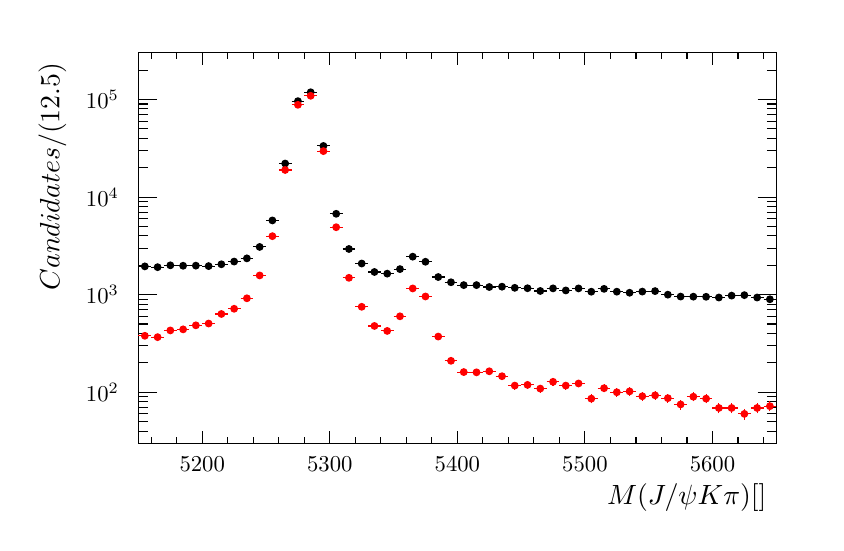
\begin{tikzpicture}
\pgfdeclareplotmark{cross} {
\pgfpathmoveto{\pgfpoint{-0.3\pgfplotmarksize}{\pgfplotmarksize}}
\pgfpathlineto{\pgfpoint{+0.3\pgfplotmarksize}{\pgfplotmarksize}}
\pgfpathlineto{\pgfpoint{+0.3\pgfplotmarksize}{0.3\pgfplotmarksize}}
\pgfpathlineto{\pgfpoint{+1\pgfplotmarksize}{0.3\pgfplotmarksize}}
\pgfpathlineto{\pgfpoint{+1\pgfplotmarksize}{-0.3\pgfplotmarksize}}
\pgfpathlineto{\pgfpoint{+0.3\pgfplotmarksize}{-0.3\pgfplotmarksize}}
\pgfpathlineto{\pgfpoint{+0.3\pgfplotmarksize}{-1.\pgfplotmarksize}}
\pgfpathlineto{\pgfpoint{-0.3\pgfplotmarksize}{-1.\pgfplotmarksize}}
\pgfpathlineto{\pgfpoint{-0.3\pgfplotmarksize}{-0.3\pgfplotmarksize}}
\pgfpathlineto{\pgfpoint{-1.\pgfplotmarksize}{-0.3\pgfplotmarksize}}
\pgfpathlineto{\pgfpoint{-1.\pgfplotmarksize}{0.3\pgfplotmarksize}}
\pgfpathlineto{\pgfpoint{-0.3\pgfplotmarksize}{0.3\pgfplotmarksize}}
\pgfpathclose
\pgfusepathqstroke
}
\pgfdeclareplotmark{cross*} {
\pgfpathmoveto{\pgfpoint{-0.3\pgfplotmarksize}{\pgfplotmarksize}}
\pgfpathlineto{\pgfpoint{+0.3\pgfplotmarksize}{\pgfplotmarksize}}
\pgfpathlineto{\pgfpoint{+0.3\pgfplotmarksize}{0.3\pgfplotmarksize}}
\pgfpathlineto{\pgfpoint{+1\pgfplotmarksize}{0.3\pgfplotmarksize}}
\pgfpathlineto{\pgfpoint{+1\pgfplotmarksize}{-0.3\pgfplotmarksize}}
\pgfpathlineto{\pgfpoint{+0.3\pgfplotmarksize}{-0.3\pgfplotmarksize}}
\pgfpathlineto{\pgfpoint{+0.3\pgfplotmarksize}{-1.\pgfplotmarksize}}
\pgfpathlineto{\pgfpoint{-0.3\pgfplotmarksize}{-1.\pgfplotmarksize}}
\pgfpathlineto{\pgfpoint{-0.3\pgfplotmarksize}{-0.3\pgfplotmarksize}}
\pgfpathlineto{\pgfpoint{-1.\pgfplotmarksize}{-0.3\pgfplotmarksize}}
\pgfpathlineto{\pgfpoint{-1.\pgfplotmarksize}{0.3\pgfplotmarksize}}
\pgfpathlineto{\pgfpoint{-0.3\pgfplotmarksize}{0.3\pgfplotmarksize}}
\pgfpathclose
\pgfusepathqfillstroke
}
\pgfdeclareplotmark{newstar} {
\pgfpathmoveto{\pgfqpoint{0pt}{\pgfplotmarksize}}
\pgfpathlineto{\pgfqpointpolar{44}{0.5\pgfplotmarksize}}
\pgfpathlineto{\pgfqpointpolar{18}{\pgfplotmarksize}}
\pgfpathlineto{\pgfqpointpolar{-20}{0.5\pgfplotmarksize}}
\pgfpathlineto{\pgfqpointpolar{-54}{\pgfplotmarksize}}
\pgfpathlineto{\pgfqpointpolar{-90}{0.5\pgfplotmarksize}}
\pgfpathlineto{\pgfqpointpolar{234}{\pgfplotmarksize}}
\pgfpathlineto{\pgfqpointpolar{198}{0.5\pgfplotmarksize}}
\pgfpathlineto{\pgfqpointpolar{162}{\pgfplotmarksize}}
\pgfpathlineto{\pgfqpointpolar{134}{0.5\pgfplotmarksize}}
\pgfpathclose
\pgfusepathqstroke
}
\pgfdeclareplotmark{newstar*} {
\pgfpathmoveto{\pgfqpoint{0pt}{\pgfplotmarksize}}
\pgfpathlineto{\pgfqpointpolar{44}{0.5\pgfplotmarksize}}
\pgfpathlineto{\pgfqpointpolar{18}{\pgfplotmarksize}}
\pgfpathlineto{\pgfqpointpolar{-20}{0.5\pgfplotmarksize}}
\pgfpathlineto{\pgfqpointpolar{-54}{\pgfplotmarksize}}
\pgfpathlineto{\pgfqpointpolar{-90}{0.5\pgfplotmarksize}}
\pgfpathlineto{\pgfqpointpolar{234}{\pgfplotmarksize}}
\pgfpathlineto{\pgfqpointpolar{198}{0.5\pgfplotmarksize}}
\pgfpathlineto{\pgfqpointpolar{162}{\pgfplotmarksize}}
\pgfpathlineto{\pgfqpointpolar{134}{0.5\pgfplotmarksize}}
\pgfpathclose
\pgfusepathqfillstroke
}
\definecolor{c}{rgb}{1,1,1};
\draw [color=c, fill=c] (0,0) rectangle (10,6.27517);
\draw [color=c, fill=c] (1.4,1.00403) rectangle (9.5,5.96141);
\definecolor{c}{rgb}{0,0,0};
\draw [c] (1.4,1.00403) -- (1.4,5.96141) -- (9.5,5.96141) -- (9.5,1.00403) -- (1.4,1.00403);
\draw [c,line width=0.4] (1.4,3.25058) -- (1.44744,3.25058);
\draw [c,line width=0.4] (1.51456,3.25058) -- (1.562,3.25058);
\foreach \P in {(1.481,3.25058)}{\draw[mark options={color=c,fill=c},mark size=1.201201pt,mark=*] plot coordinates {\P};}
\draw [c,line width=0.4] (1.562,3.24054) -- (1.60944,3.24054);
\draw [c,line width=0.4] (1.67656,3.24054) -- (1.724,3.24054);
\foreach \P in {(1.643,3.24054)}{\draw[mark options={color=c,fill=c},mark size=1.201201pt,mark=*] plot coordinates {\P};}
\draw [c,line width=0.4] (1.724,3.26421) -- (1.77144,3.26421);
\draw [c,line width=0.4] (1.83856,3.26421) -- (1.886,3.26421);
\foreach \P in {(1.805,3.26421)}{\draw[mark options={color=c,fill=c},mark size=1.201201pt,mark=*] plot coordinates {\P};}
\draw [c,line width=0.4] (1.886,3.25853) -- (1.93344,3.25853);
\draw [c,line width=0.4] (2.00056,3.25853) -- (2.048,3.25853);
\foreach \P in {(1.967,3.25853)}{\draw[mark options={color=c,fill=c},mark size=1.201201pt,mark=*] plot coordinates {\P};}
\draw [c,line width=0.4] (2.048,3.25989) -- (2.09544,3.25989);
\draw [c,line width=0.4] (2.16256,3.25989) -- (2.21,3.25989);
\foreach \P in {(2.129,3.25989)}{\draw[mark options={color=c,fill=c},mark size=1.201201pt,mark=*] plot coordinates {\P};}
\draw [c,line width=0.4] (2.21,3.25416) -- (2.25744,3.25416);
\draw [c,line width=0.4] (2.32456,3.25416) -- (2.372,3.25416);
\foreach \P in {(2.291,3.25416)}{\draw[mark options={color=c,fill=c},mark size=1.201201pt,mark=*] plot coordinates {\P};}
\draw [c,line width=0.4] (2.372,3.27725) -- (2.41944,3.27725);
\draw [c,line width=0.4] (2.48656,3.27725) -- (2.534,3.27725);
\foreach \P in {(2.453,3.27725)}{\draw[mark options={color=c,fill=c},mark size=1.201201pt,mark=*] plot coordinates {\P};}
\draw [c,line width=0.4] (2.534,3.3116) -- (2.58144,3.3116);
\draw [c,line width=0.4] (2.64856,3.3116) -- (2.696,3.3116);
\foreach \P in {(2.615,3.3116)}{\draw[mark options={color=c,fill=c},mark size=1.201201pt,mark=*] plot coordinates {\P};}
\draw [c,line width=0.4] (2.696,3.35243) -- (2.74344,3.35243);
\draw [c,line width=0.4] (2.81056,3.35243) -- (2.858,3.35243);
\foreach \P in {(2.777,3.35243)}{\draw[mark options={color=c,fill=c},mark size=1.201201pt,mark=*] plot coordinates {\P};}
\draw [c,line width=0.4] (2.858,3.49741) -- (2.90544,3.49741);
\draw [c,line width=0.4] (2.97256,3.49741) -- (3.02,3.49741);
\foreach \P in {(2.939,3.49741)}{\draw[mark options={color=c,fill=c},mark size=1.201201pt,mark=*] plot coordinates {\P};}
\draw [c,line width=0.4] (3.02,3.83411) -- (3.06744,3.83411);
\draw [c,line width=0.4] (3.13456,3.83411) -- (3.182,3.83411);
\foreach \P in {(3.101,3.83411)}{\draw[mark options={color=c,fill=c},mark size=1.201201pt,mark=*] plot coordinates {\P};}
\draw [c,line width=0.4] (3.182,4.55666) -- (3.22944,4.55666);
\draw [c,line width=0.4] (3.29656,4.55666) -- (3.344,4.55666);
\foreach \P in {(3.263,4.55666)}{\draw[mark options={color=c,fill=c},mark size=1.201201pt,mark=*] plot coordinates {\P};}
\draw [c,line width=0.4] (3.344,5.34895) -- (3.39144,5.34895);
\draw [c,line width=0.4] (3.45856,5.34895) -- (3.506,5.34895);
\foreach \P in {(3.425,5.34895)}{\draw[mark options={color=c,fill=c},mark size=1.201201pt,mark=*] plot coordinates {\P};}
\draw [c,line width=0.4] (3.506,5.46194) -- (3.55344,5.46194);
\draw [c,line width=0.4] (3.62056,5.46194) -- (3.668,5.46194);
\foreach \P in {(3.587,5.46194)}{\draw[mark options={color=c,fill=c},mark size=1.201201pt,mark=*] plot coordinates {\P};}
\draw [c,line width=0.4] (3.668,4.78019) -- (3.71544,4.78019);
\draw [c,line width=0.4] (3.78256,4.78019) -- (3.83,4.78019);
\foreach \P in {(3.749,4.78019)}{\draw[mark options={color=c,fill=c},mark size=1.201201pt,mark=*] plot coordinates {\P};}
\draw [c,line width=0.4] (3.83,3.9184) -- (3.87744,3.9184);
\draw [c,line width=0.4] (3.94456,3.9184) -- (3.992,3.9184);
\foreach \P in {(3.911,3.9184)}{\draw[mark options={color=c,fill=c},mark size=1.201201pt,mark=*] plot coordinates {\P};}
\draw [c,line width=0.4] (3.992,3.47166) -- (4.03944,3.47166);
\draw [c,line width=0.4] (4.10656,3.47166) -- (4.154,3.47166);
\foreach \P in {(4.073,3.47166)}{\draw[mark options={color=c,fill=c},mark size=1.201201pt,mark=*] plot coordinates {\P};}
\draw [c,line width=0.4] (4.154,3.28688) -- (4.20144,3.28688);
\draw [c,line width=0.4] (4.26856,3.28688) -- (4.316,3.28688);
\foreach \P in {(4.235,3.28688)}{\draw[mark options={color=c,fill=c},mark size=1.201201pt,mark=*] plot coordinates {\P};}
\draw [c,line width=0.4] (4.316,3.17953) -- (4.36344,3.17953);
\draw [c,line width=0.4] (4.43056,3.17953) -- (4.478,3.17953);
\foreach \P in {(4.397,3.17953)}{\draw[mark options={color=c,fill=c},mark size=1.201201pt,mark=*] plot coordinates {\P};}
\draw [c,line width=0.4] (4.478,3.15832) -- (4.52544,3.15832);
\draw [c,line width=0.4] (4.59256,3.15832) -- (4.64,3.15832);
\foreach \P in {(4.559,3.15832)}{\draw[mark options={color=c,fill=c},mark size=1.201201pt,mark=*] plot coordinates {\P};}
\draw [c,line width=0.4] (4.64,3.21608) -- (4.68744,3.21608);
\draw [c,line width=0.4] (4.75456,3.21608) -- (4.802,3.21608);
\foreach \P in {(4.721,3.21608)}{\draw[mark options={color=c,fill=c},mark size=1.201201pt,mark=*] plot coordinates {\P};}
\draw [c,line width=0.4] (4.802,3.37393) -- (4.84944,3.37393);
\draw [c,line width=0.4] (4.91656,3.37393) -- (4.964,3.37393);
\foreach \P in {(4.883,3.37393)}{\draw[mark options={color=c,fill=c},mark size=1.201201pt,mark=*] plot coordinates {\P};}
\draw [c,line width=0.4] (4.964,3.30938) -- (5.01144,3.30938);
\draw [c,line width=0.4] (5.07856,3.30938) -- (5.126,3.30938);
\foreach \P in {(5.045,3.30938)}{\draw[mark options={color=c,fill=c},mark size=1.201201pt,mark=*] plot coordinates {\P};}
\draw [c,line width=0.4] (5.126,3.11535) -- (5.17344,3.11535);
\draw [c,line width=0.4] (5.24056,3.11535) -- (5.288,3.11535);
\foreach \P in {(5.207,3.11535)}{\draw[mark options={color=c,fill=c},mark size=1.201201pt,mark=*] plot coordinates {\P};}
\draw [c,line width=0.4] (5.288,3.04893) -- (5.33544,3.04893);
\draw [c,line width=0.4] (5.40256,3.04893) -- (5.45,3.04893);
\foreach \P in {(5.369,3.04893)}{\draw[mark options={color=c,fill=c},mark size=1.201201pt,mark=*] plot coordinates {\P};}
\draw [c,line width=0.4] (5.45,3.0128) -- (5.49744,3.0128);
\draw [c,line width=0.4] (5.56456,3.0128) -- (5.612,3.0128);
\foreach \P in {(5.531,3.0128)}{\draw[mark options={color=c,fill=c},mark size=1.201201pt,mark=*] plot coordinates {\P};}
\draw [c,line width=0.4] (5.612,3.0128) -- (5.65944,3.0128);
\draw [c,line width=0.4] (5.72656,3.0128) -- (5.774,3.0128);
\foreach \P in {(5.693,3.0128)}{\draw[mark options={color=c,fill=c},mark size=1.201201pt,mark=*] plot coordinates {\P};}
\draw [c,line width=0.4] (5.774,2.98864) -- (5.82144,2.98864);
\draw [c,line width=0.4] (5.88856,2.98864) -- (5.936,2.98864);
\foreach \P in {(5.855,2.98864)}{\draw[mark options={color=c,fill=c},mark size=1.201201pt,mark=*] plot coordinates {\P};}
\draw [c,line width=0.4] (5.936,2.99266) -- (5.98344,2.99266);
\draw [c,line width=0.4] (6.05056,2.99266) -- (6.098,2.99266);
\foreach \P in {(6.017,2.99266)}{\draw[mark options={color=c,fill=c},mark size=1.201201pt,mark=*] plot coordinates {\P};}
\draw [c,line width=0.4] (6.098,2.9782) -- (6.14544,2.9782);
\draw [c,line width=0.4] (6.21256,2.9782) -- (6.26,2.9782);
\foreach \P in {(6.179,2.9782)}{\draw[mark options={color=c,fill=c},mark size=1.201201pt,mark=*] plot coordinates {\P};}
\draw [c,line width=0.4] (6.26,2.97314) -- (6.30744,2.97314);
\draw [c,line width=0.4] (6.37456,2.97314) -- (6.422,2.97314);
\foreach \P in {(6.341,2.97314)}{\draw[mark options={color=c,fill=c},mark size=1.201201pt,mark=*] plot coordinates {\P};}
\draw [c,line width=0.4] (6.422,2.93828) -- (6.46944,2.93828);
\draw [c,line width=0.4] (6.53656,2.93828) -- (6.584,2.93828);
\foreach \P in {(6.503,2.93828)}{\draw[mark options={color=c,fill=c},mark size=1.201201pt,mark=*] plot coordinates {\P};}
\draw [c,line width=0.4] (6.584,2.97129) -- (6.63144,2.97129);
\draw [c,line width=0.4] (6.69856,2.97129) -- (6.746,2.97129);
\foreach \P in {(6.665,2.97129)}{\draw[mark options={color=c,fill=c},mark size=1.201201pt,mark=*] plot coordinates {\P};}
\draw [c,line width=0.4] (6.746,2.94514) -- (6.79344,2.94514);
\draw [c,line width=0.4] (6.86056,2.94514) -- (6.908,2.94514);
\foreach \P in {(6.827,2.94514)}{\draw[mark options={color=c,fill=c},mark size=1.201201pt,mark=*] plot coordinates {\P};}
\draw [c,line width=0.4] (6.908,2.97082) -- (6.95544,2.97082);
\draw [c,line width=0.4] (7.02256,2.97082) -- (7.07,2.97082);
\foreach \P in {(6.989,2.97082)}{\draw[mark options={color=c,fill=c},mark size=1.201201pt,mark=*] plot coordinates {\P};}
\draw [c,line width=0.4] (7.07,2.92882) -- (7.11744,2.92882);
\draw [c,line width=0.4] (7.18456,2.92882) -- (7.232,2.92882);
\foreach \P in {(7.151,2.92882)}{\draw[mark options={color=c,fill=c},mark size=1.201201pt,mark=*] plot coordinates {\P};}
\draw [c,line width=0.4] (7.232,2.96522) -- (7.27944,2.96522);
\draw [c,line width=0.4] (7.34656,2.96522) -- (7.394,2.96522);
\foreach \P in {(7.313,2.96522)}{\draw[mark options={color=c,fill=c},mark size=1.201201pt,mark=*] plot coordinates {\P};}
\draw [c,line width=0.4] (7.394,2.92932) -- (7.44144,2.92932);
\draw [c,line width=0.4] (7.50856,2.92932) -- (7.556,2.92932);
\foreach \P in {(7.475,2.92932)}{\draw[mark options={color=c,fill=c},mark size=1.201201pt,mark=*] plot coordinates {\P};}
\draw [c,line width=0.4] (7.556,2.91561) -- (7.60344,2.91561);
\draw [c,line width=0.4] (7.67056,2.91561) -- (7.718,2.91561);
\foreach \P in {(7.637,2.91561)}{\draw[mark options={color=c,fill=c},mark size=1.201201pt,mark=*] plot coordinates {\P};}
\draw [c,line width=0.4] (7.718,2.93033) -- (7.76544,2.93033);
\draw [c,line width=0.4] (7.83256,2.93033) -- (7.88,2.93033);
\foreach \P in {(7.799,2.93033)}{\draw[mark options={color=c,fill=c},mark size=1.201201pt,mark=*] plot coordinates {\P};}
\draw [c,line width=0.4] (7.88,2.9368) -- (7.92744,2.9368);
\draw [c,line width=0.4] (7.99456,2.9368) -- (8.042,2.9368);
\foreach \P in {(7.961,2.9368)}{\draw[mark options={color=c,fill=c},mark size=1.201201pt,mark=*] plot coordinates {\P};}
\draw [c,line width=0.4] (8.042,2.8914) -- (8.08944,2.8914);
\draw [c,line width=0.4] (8.15656,2.8914) -- (8.204,2.8914);
\foreach \P in {(8.123,2.8914)}{\draw[mark options={color=c,fill=c},mark size=1.201201pt,mark=*] plot coordinates {\P};}
\draw [c,line width=0.4] (8.204,2.86718) -- (8.25144,2.86718);
\draw [c,line width=0.4] (8.31856,2.86718) -- (8.366,2.86718);
\foreach \P in {(8.285,2.86718)}{\draw[mark options={color=c,fill=c},mark size=1.201201pt,mark=*] plot coordinates {\P};}
\draw [c,line width=0.4] (8.366,2.86605) -- (8.41344,2.86605);
\draw [c,line width=0.4] (8.48056,2.86605) -- (8.528,2.86605);
\foreach \P in {(8.447,2.86605)}{\draw[mark options={color=c,fill=c},mark size=1.201201pt,mark=*] plot coordinates {\P};}
\draw [c,line width=0.4] (8.528,2.86436) -- (8.57544,2.86436);
\draw [c,line width=0.4] (8.64256,2.86436) -- (8.69,2.86436);
\foreach \P in {(8.609,2.86436)}{\draw[mark options={color=c,fill=c},mark size=1.201201pt,mark=*] plot coordinates {\P};}
\draw [c,line width=0.4] (8.69,2.85523) -- (8.73744,2.85523);
\draw [c,line width=0.4] (8.80456,2.85523) -- (8.852,2.85523);
\foreach \P in {(8.771,2.85523)}{\draw[mark options={color=c,fill=c},mark size=1.201201pt,mark=*] plot coordinates {\P};}
\draw [c,line width=0.4] (8.852,2.87943) -- (8.89944,2.87943);
\draw [c,line width=0.4] (8.96656,2.87943) -- (9.014,2.87943);
\foreach \P in {(8.933,2.87943)}{\draw[mark options={color=c,fill=c},mark size=1.201201pt,mark=*] plot coordinates {\P};}
\draw [c,line width=0.4] (9.014,2.88545) -- (9.06144,2.88545);
\draw [c,line width=0.4] (9.12856,2.88545) -- (9.176,2.88545);
\foreach \P in {(9.095,2.88545)}{\draw[mark options={color=c,fill=c},mark size=1.201201pt,mark=*] plot coordinates {\P};}
\draw [c,line width=0.4] (9.176,2.85523) -- (9.22344,2.85523);
\draw [c,line width=0.4] (9.29056,2.85523) -- (9.338,2.85523);
\foreach \P in {(9.257,2.85523)}{\draw[mark options={color=c,fill=c},mark size=1.201201pt,mark=*] plot coordinates {\P};}
\draw [c,line width=0.4] (9.338,2.83289) -- (9.38544,2.83289);
\draw [c,line width=0.4] (9.45256,2.83289) -- (9.5,2.83289);
\foreach \P in {(9.419,2.83289)}{\draw[mark options={color=c,fill=c},mark size=1.201201pt,mark=*] plot coordinates {\P};}
\draw [c,line width=0.4] (1.4,1.00403) -- (9.5,1.00403);
\draw [anchor= east] (9.5,0.317272) node[scale=1.00614, rotate=0]{$\text{M}(J/\psi K\pi)  [\mevcc]$};
\draw [c,line width=0.4] (2.21,1.15651) -- (2.21,1.00403);
\draw [c,line width=0.4] (2.534,1.08027) -- (2.534,1.00403);
\draw [c,line width=0.4] (2.858,1.08027) -- (2.858,1.00403);
\draw [c,line width=0.4] (3.182,1.08027) -- (3.182,1.00403);
\draw [c,line width=0.4] (3.506,1.08027) -- (3.506,1.00403);
\draw [c,line width=0.4] (3.83,1.15651) -- (3.83,1.00403);
\draw [c,line width=0.4] (4.154,1.08027) -- (4.154,1.00403);
\draw [c,line width=0.4] (4.478,1.08027) -- (4.478,1.00403);
\draw [c,line width=0.4] (4.802,1.08027) -- (4.802,1.00403);
\draw [c,line width=0.4] (5.126,1.08027) -- (5.126,1.00403);
\draw [c,line width=0.4] (5.45,1.15651) -- (5.45,1.00403);
\draw [c,line width=0.4] (5.774,1.08027) -- (5.774,1.00403);
\draw [c,line width=0.4] (6.098,1.08027) -- (6.098,1.00403);
\draw [c,line width=0.4] (6.422,1.08027) -- (6.422,1.00403);
\draw [c,line width=0.4] (6.746,1.08027) -- (6.746,1.00403);
\draw [c,line width=0.4] (7.07,1.15651) -- (7.07,1.00403);
\draw [c,line width=0.4] (7.394,1.08027) -- (7.394,1.00403);
\draw [c,line width=0.4] (7.718,1.08027) -- (7.718,1.00403);
\draw [c,line width=0.4] (8.042,1.08027) -- (8.042,1.00403);
\draw [c,line width=0.4] (8.366,1.08027) -- (8.366,1.00403);
\draw [c,line width=0.4] (8.69,1.15651) -- (8.69,1.00403);
\draw [c,line width=0.4] (2.21,1.15651) -- (2.21,1.00403);
\draw [c,line width=0.4] (1.886,1.08027) -- (1.886,1.00403);
\draw [c,line width=0.4] (1.562,1.08027) -- (1.562,1.00403);
\draw [c,line width=0.4] (8.69,1.15651) -- (8.69,1.00403);
\draw [c,line width=0.4] (9.014,1.08027) -- (9.014,1.00403);
\draw [c,line width=0.4] (9.338,1.08027) -- (9.338,1.00403);
\draw [anchor=base] (2.21,0.640067) node[scale=0.819821, rotate=0]{5200};
\draw [anchor=base] (3.83,0.640067) node[scale=0.819821, rotate=0]{5300};
\draw [anchor=base] (5.45,0.640067) node[scale=0.819821, rotate=0]{5400};
\draw [anchor=base] (7.07,0.640067) node[scale=0.819821, rotate=0]{5500};
\draw [anchor=base] (8.69,0.640067) node[scale=0.819821, rotate=0]{5600};
\draw [c,line width=0.4] (1.4,5.96141) -- (9.5,5.96141);
\draw [c,line width=0.4] (2.21,5.80892) -- (2.21,5.96141);
\draw [c,line width=0.4] (2.534,5.88517) -- (2.534,5.96141);
\draw [c,line width=0.4] (2.858,5.88517) -- (2.858,5.96141);
\draw [c,line width=0.4] (3.182,5.88517) -- (3.182,5.96141);
\draw [c,line width=0.4] (3.506,5.88517) -- (3.506,5.96141);
\draw [c,line width=0.4] (3.83,5.80892) -- (3.83,5.96141);
\draw [c,line width=0.4] (4.154,5.88517) -- (4.154,5.96141);
\draw [c,line width=0.4] (4.478,5.88517) -- (4.478,5.96141);
\draw [c,line width=0.4] (4.802,5.88517) -- (4.802,5.96141);
\draw [c,line width=0.4] (5.126,5.88517) -- (5.126,5.96141);
\draw [c,line width=0.4] (5.45,5.80892) -- (5.45,5.96141);
\draw [c,line width=0.4] (5.774,5.88517) -- (5.774,5.96141);
\draw [c,line width=0.4] (6.098,5.88517) -- (6.098,5.96141);
\draw [c,line width=0.4] (6.422,5.88517) -- (6.422,5.96141);
\draw [c,line width=0.4] (6.746,5.88517) -- (6.746,5.96141);
\draw [c,line width=0.4] (7.07,5.80892) -- (7.07,5.96141);
\draw [c,line width=0.4] (7.394,5.88517) -- (7.394,5.96141);
\draw [c,line width=0.4] (7.718,5.88517) -- (7.718,5.96141);
\draw [c,line width=0.4] (8.042,5.88517) -- (8.042,5.96141);
\draw [c,line width=0.4] (8.366,5.88517) -- (8.366,5.96141);
\draw [c,line width=0.4] (8.69,5.80892) -- (8.69,5.96141);
\draw [c,line width=0.4] (2.21,5.80892) -- (2.21,5.96141);
\draw [c,line width=0.4] (1.886,5.88517) -- (1.886,5.96141);
\draw [c,line width=0.4] (1.562,5.88517) -- (1.562,5.96141);
\draw [c,line width=0.4] (8.69,5.80892) -- (8.69,5.96141);
\draw [c,line width=0.4] (9.014,5.88517) -- (9.014,5.96141);
\draw [c,line width=0.4] (9.338,5.88517) -- (9.338,5.96141);
\draw [c,line width=0.4] (1.4,1.00403) -- (1.4,5.96141);
\draw [anchor= east] (0.3056,5.96141) node[scale=1.00614, rotate=90]{$\text{Candidates} / (12.5 \mevcc)$};
\draw [c,line width=0.4] (1.5185,1.15887) -- (1.4,1.15887);
\draw [c,line width=0.4] (1.5185,1.27897) -- (1.4,1.27897);
\draw [c,line width=0.4] (1.5185,1.37711) -- (1.4,1.37711);
\draw [c,line width=0.4] (1.5185,1.46008) -- (1.4,1.46008);
\draw [c,line width=0.4] (1.5185,1.53195) -- (1.4,1.53195);
\draw [c,line width=0.4] (1.5185,1.59534) -- (1.4,1.59534);
\draw [c,line width=0.4] (1.637,1.65205) -- (1.4,1.65205);
\draw [anchor= east] (1.252,1.65205) node[scale=0.819821, rotate=0]{$10^{2}$};
\draw [c,line width=0.4] (1.5185,2.02513) -- (1.4,2.02513);
\draw [c,line width=0.4] (1.5185,2.24337) -- (1.4,2.24337);
\draw [c,line width=0.4] (1.5185,2.39821) -- (1.4,2.39821);
\draw [c,line width=0.4] (1.5185,2.51832) -- (1.4,2.51832);
\draw [c,line width=0.4] (1.5185,2.61645) -- (1.4,2.61645);
\draw [c,line width=0.4] (1.5185,2.69942) -- (1.4,2.69942);
\draw [c,line width=0.4] (1.5185,2.77129) -- (1.4,2.77129);
\draw [c,line width=0.4] (1.5185,2.83469) -- (1.4,2.83469);
\draw [c,line width=0.4] (1.637,2.8914) -- (1.4,2.8914);
\draw [anchor= east] (1.252,2.8914) node[scale=0.819821, rotate=0]{$10^{3}$};
\draw [c,line width=0.4] (1.5185,3.26448) -- (1.4,3.26448);
\draw [c,line width=0.4] (1.5185,3.48272) -- (1.4,3.48272);
\draw [c,line width=0.4] (1.5185,3.63756) -- (1.4,3.63756);
\draw [c,line width=0.4] (1.5185,3.75766) -- (1.4,3.75766);
\draw [c,line width=0.4] (1.5185,3.8558) -- (1.4,3.8558);
\draw [c,line width=0.4] (1.5185,3.93877) -- (1.4,3.93877);
\draw [c,line width=0.4] (1.5185,4.01064) -- (1.4,4.01064);
\draw [c,line width=0.4] (1.5185,4.07404) -- (1.4,4.07404);
\draw [c,line width=0.4] (1.637,4.13075) -- (1.4,4.13075);
\draw [anchor= east] (1.252,4.13075) node[scale=0.819821, rotate=0]{$10^{4}$};
\draw [c,line width=0.4] (1.5185,4.50383) -- (1.4,4.50383);
\draw [c,line width=0.4] (1.5185,4.72206) -- (1.4,4.72206);
\draw [c,line width=0.4] (1.5185,4.87691) -- (1.4,4.87691);
\draw [c,line width=0.4] (1.5185,4.99701) -- (1.4,4.99701);
\draw [c,line width=0.4] (1.5185,5.09514) -- (1.4,5.09514);
\draw [c,line width=0.4] (1.5185,5.17811) -- (1.4,5.17811);
\draw [c,line width=0.4] (1.5185,5.24999) -- (1.4,5.24999);
\draw [c,line width=0.4] (1.5185,5.31338) -- (1.4,5.31338);
\draw [c,line width=0.4] (1.637,5.37009) -- (1.4,5.37009);
\draw [anchor= east] (1.252,5.37009) node[scale=0.819821, rotate=0]{$10^{5}$};
\draw [c,line width=0.4] (1.5185,5.74317) -- (1.4,5.74317);
\draw [c,line width=0.4] (1.5185,5.96141) -- (1.4,5.96141);
\draw [c,line width=0.4] (9.5,1.00403) -- (9.5,5.96141);
\draw [c,line width=0.4] (9.3815,1.15887) -- (9.5,1.15887);
\draw [c,line width=0.4] (9.3815,1.27897) -- (9.5,1.27897);
\draw [c,line width=0.4] (9.3815,1.37711) -- (9.5,1.37711);
\draw [c,line width=0.4] (9.3815,1.46008) -- (9.5,1.46008);
\draw [c,line width=0.4] (9.3815,1.53195) -- (9.5,1.53195);
\draw [c,line width=0.4] (9.3815,1.59534) -- (9.5,1.59534);
\draw [c,line width=0.4] (9.263,1.65205) -- (9.5,1.65205);
\draw [c,line width=0.4] (9.3815,2.02513) -- (9.5,2.02513);
\draw [c,line width=0.4] (9.3815,2.24337) -- (9.5,2.24337);
\draw [c,line width=0.4] (9.3815,2.39821) -- (9.5,2.39821);
\draw [c,line width=0.4] (9.3815,2.51832) -- (9.5,2.51832);
\draw [c,line width=0.4] (9.3815,2.61645) -- (9.5,2.61645);
\draw [c,line width=0.4] (9.3815,2.69942) -- (9.5,2.69942);
\draw [c,line width=0.4] (9.3815,2.77129) -- (9.5,2.77129);
\draw [c,line width=0.4] (9.3815,2.83469) -- (9.5,2.83469);
\draw [c,line width=0.4] (9.263,2.8914) -- (9.5,2.8914);
\draw [c,line width=0.4] (9.3815,3.26448) -- (9.5,3.26448);
\draw [c,line width=0.4] (9.3815,3.48272) -- (9.5,3.48272);
\draw [c,line width=0.4] (9.3815,3.63756) -- (9.5,3.63756);
\draw [c,line width=0.4] (9.3815,3.75766) -- (9.5,3.75766);
\draw [c,line width=0.4] (9.3815,3.8558) -- (9.5,3.8558);
\draw [c,line width=0.4] (9.3815,3.93877) -- (9.5,3.93877);
\draw [c,line width=0.4] (9.3815,4.01064) -- (9.5,4.01064);
\draw [c,line width=0.4] (9.3815,4.07404) -- (9.5,4.07404);
\draw [c,line width=0.4] (9.263,4.13075) -- (9.5,4.13075);
\draw [c,line width=0.4] (9.3815,4.50383) -- (9.5,4.50383);
\draw [c,line width=0.4] (9.3815,4.72206) -- (9.5,4.72206);
\draw [c,line width=0.4] (9.3815,4.87691) -- (9.5,4.87691);
\draw [c,line width=0.4] (9.3815,4.99701) -- (9.5,4.99701);
\draw [c,line width=0.4] (9.3815,5.09514) -- (9.5,5.09514);
\draw [c,line width=0.4] (9.3815,5.17811) -- (9.5,5.17811);
\draw [c,line width=0.4] (9.3815,5.24999) -- (9.5,5.24999);
\draw [c,line width=0.4] (9.3815,5.31338) -- (9.5,5.31338);
\draw [c,line width=0.4] (9.263,5.37009) -- (9.5,5.37009);
\draw [c,line width=0.4] (9.3815,5.74317) -- (9.5,5.74317);
\draw [c,line width=0.4] (9.3815,5.96141) -- (9.5,5.96141);
\definecolor{c}{rgb}{1,0,0};
\draw [c,line width=0.4] (1.4,2.36919) -- (1.44744,2.36919);
\draw [c,line width=0.4] (1.51456,2.36919) -- (1.562,2.36919);
\foreach \P in {(1.481,2.36919)}{\draw[mark options={color=c,fill=c},mark size=1.201201pt,mark=*] plot coordinates {\P};}
\draw [c,line width=0.4] (1.562,2.35187) -- (1.60944,2.35187);
\draw [c,line width=0.4] (1.67656,2.35187) -- (1.724,2.35187);
\foreach \P in {(1.643,2.35187)}{\draw[mark options={color=c,fill=c},mark size=1.201201pt,mark=*] plot coordinates {\P};}
\draw [c,line width=0.4] (1.724,2.43714) -- (1.77144,2.43714);
\draw [c,line width=0.4] (1.83856,2.43714) -- (1.886,2.43714);
\foreach \P in {(1.805,2.43714)}{\draw[mark options={color=c,fill=c},mark size=1.201201pt,mark=*] plot coordinates {\P};}
\draw [c,line width=0.4] (1.886,2.45074) -- (1.93344,2.45074);
\draw [c,line width=0.4] (2.00056,2.45074) -- (2.048,2.45074);
\foreach \P in {(1.967,2.45074)}{\draw[mark options={color=c,fill=c},mark size=1.201201pt,mark=*] plot coordinates {\P};}
\draw [c,line width=0.4] (2.048,2.50193) -- (2.09544,2.50193);
\draw [c,line width=0.4] (2.16256,2.50193) -- (2.21,2.50193);
\foreach \P in {(2.129,2.50193)}{\draw[mark options={color=c,fill=c},mark size=1.201201pt,mark=*] plot coordinates {\P};}
\draw [c,line width=0.4] (2.21,2.52474) -- (2.25744,2.52474);
\draw [c,line width=0.4] (2.32456,2.52474) -- (2.372,2.52474);
\foreach \P in {(2.291,2.52474)}{\draw[mark options={color=c,fill=c},mark size=1.201201pt,mark=*] plot coordinates {\P};}
\draw [c,line width=0.4] (2.372,2.64612) -- (2.41944,2.64612);
\draw [c,line width=0.4] (2.48656,2.64612) -- (2.534,2.64612);
\foreach \P in {(2.453,2.64612)}{\draw[mark options={color=c,fill=c},mark size=1.201201pt,mark=*] plot coordinates {\P};}
\draw [c,line width=0.4] (2.534,2.71234) -- (2.58144,2.71234);
\draw [c,line width=0.4] (2.64856,2.71234) -- (2.696,2.71234);
\foreach \P in {(2.615,2.71234)}{\draw[mark options={color=c,fill=c},mark size=1.201201pt,mark=*] plot coordinates {\P};}
\draw [c,line width=0.4] (2.696,2.84535) -- (2.74344,2.84535);
\draw [c,line width=0.4] (2.81056,2.84535) -- (2.858,2.84535);
\foreach \P in {(2.777,2.84535)}{\draw[mark options={color=c,fill=c},mark size=1.201201pt,mark=*] plot coordinates {\P};}
\draw [c,line width=0.4] (2.858,3.13556) -- (2.90544,3.13556);
\draw [c,line width=0.4] (2.97256,3.13556) -- (3.02,3.13556);
\foreach \P in {(2.939,3.13556)}{\draw[mark options={color=c,fill=c},mark size=1.201201pt,mark=*] plot coordinates {\P};}
\draw [c,line width=0.4] (3.02,3.63432) -- (3.06744,3.63432);
\draw [c,line width=0.4] (3.13456,3.63432) -- (3.182,3.63432);
\foreach \P in {(3.101,3.63432)}{\draw[mark options={color=c,fill=c},mark size=1.201201pt,mark=*] plot coordinates {\P};}
\draw [c,line width=0.4] (3.182,4.47494) -- (3.22944,4.47494);
\draw [c,line width=0.4] (3.29656,4.47494) -- (3.344,4.47494);
\foreach \P in {(3.263,4.47494)}{\draw[mark options={color=c,fill=c},mark size=1.201201pt,mark=*] plot coordinates {\P};}
\draw [c,line width=0.4] (3.344,5.30249) -- (3.39144,5.30249);
\draw [c,line width=0.4] (3.45856,5.30249) -- (3.506,5.30249);
\foreach \P in {(3.425,5.30249)}{\draw[mark options={color=c,fill=c},mark size=1.201201pt,mark=*] plot coordinates {\P};}
\draw [c,line width=0.4] (3.506,5.4168) -- (3.55344,5.4168);
\draw [c,line width=0.4] (3.62056,5.4168) -- (3.668,5.4168);
\foreach \P in {(3.587,5.4168)}{\draw[mark options={color=c,fill=c},mark size=1.201201pt,mark=*] plot coordinates {\P};}
\draw [c,line width=0.4] (3.668,4.71451) -- (3.71544,4.71451);
\draw [c,line width=0.4] (3.78256,4.71451) -- (3.83,4.71451);
\foreach \P in {(3.749,4.71451)}{\draw[mark options={color=c,fill=c},mark size=1.201201pt,mark=*] plot coordinates {\P};}
\draw [c,line width=0.4] (3.83,3.748) -- (3.87744,3.748);
\draw [c,line width=0.4] (3.94456,3.748) -- (3.992,3.748);
\foreach \P in {(3.911,3.748)}{\draw[mark options={color=c,fill=c},mark size=1.201201pt,mark=*] plot coordinates {\P};}
\draw [c,line width=0.4] (3.992,3.10531) -- (4.03944,3.10531);
\draw [c,line width=0.4] (4.10656,3.10531) -- (4.154,3.10531);
\foreach \P in {(4.073,3.10531)}{\draw[mark options={color=c,fill=c},mark size=1.201201pt,mark=*] plot coordinates {\P};}
\draw [c,line width=0.4] (4.154,2.73727) -- (4.20144,2.73727);
\draw [c,line width=0.4] (4.26856,2.73727) -- (4.316,2.73727);
\foreach \P in {(4.235,2.73727)}{\draw[mark options={color=c,fill=c},mark size=1.201201pt,mark=*] plot coordinates {\P};}
\draw [c,line width=0.4] (4.316,2.4941) -- (4.36344,2.4941);
\draw [c,line width=0.4] (4.43056,2.4941) -- (4.478,2.4941);
\foreach \P in {(4.397,2.4941)}{\draw[mark options={color=c,fill=c},mark size=1.201201pt,mark=*] plot coordinates {\P};}
\draw [c,line width=0.4] (4.478,2.43085) -- (4.52544,2.43085);
\draw [c,line width=0.4] (4.59256,2.43085) -- (4.64,2.43085);
\foreach \P in {(4.559,2.43085)}{\draw[mark options={color=c,fill=c},mark size=1.201201pt,mark=*] plot coordinates {\P};}
\draw [c,line width=0.4] (4.64,2.61645) -- (4.68744,2.61645);
\draw [c,line width=0.4] (4.75456,2.61645) -- (4.802,2.61645);
\foreach \P in {(4.721,2.61645)}{\draw[mark options={color=c,fill=c},mark size=1.201201pt,mark=*] plot coordinates {\P};}
\draw [c,line width=0.4] (4.802,2.97036) -- (4.84944,2.97036);
\draw [c,line width=0.4] (4.91656,2.97036) -- (4.964,2.97036);
\foreach \P in {(4.883,2.97036)}{\draw[mark options={color=c,fill=c},mark size=1.201201pt,mark=*] plot coordinates {\P};}
\draw [c,line width=0.4] (4.964,2.86831) -- (5.01144,2.86831);
\draw [c,line width=0.4] (5.07856,2.86831) -- (5.126,2.86831);
\foreach \P in {(5.045,2.86831)}{\draw[mark options={color=c,fill=c},mark size=1.201201pt,mark=*] plot coordinates {\P};}
\draw [c,line width=0.4] (5.126,2.35915) -- (5.17344,2.35915);
\draw [c,line width=0.4] (5.24056,2.35915) -- (5.288,2.35915);
\foreach \P in {(5.207,2.35915)}{\draw[mark options={color=c,fill=c},mark size=1.201201pt,mark=*] plot coordinates {\P};}
\draw [c,line width=0.4] (5.369,2.01291) -- (5.369,2.01784);
\draw [c,line width=0.4] (5.369,2.08495) -- (5.369,2.08731);
\draw [c,line width=0.4] (5.288,2.0514) -- (5.33544,2.0514);
\draw [c,line width=0.4] (5.40256,2.0514) -- (5.45,2.0514);
\foreach \P in {(5.369,2.0514)}{\draw[mark options={color=c,fill=c},mark size=1.201201pt,mark=*] plot coordinates {\P};}
\draw [c,line width=0.4] (5.531,1.8642) -- (5.531,1.87483);
\draw [c,line width=0.4] (5.531,1.94194) -- (5.531,1.94921);
\draw [c,line width=0.4] (5.45,1.90838) -- (5.49744,1.90838);
\draw [c,line width=0.4] (5.56456,1.90838) -- (5.612,1.90838);
\foreach \P in {(5.531,1.90838)}{\draw[mark options={color=c,fill=c},mark size=1.201201pt,mark=*] plot coordinates {\P};}
\draw [c,line width=0.4] (5.693,1.8607) -- (5.693,1.87147);
\draw [c,line width=0.4] (5.693,1.93859) -- (5.693,1.94598);
\draw [c,line width=0.4] (5.612,1.90503) -- (5.65944,1.90503);
\draw [c,line width=0.4] (5.72656,1.90503) -- (5.774,1.90503);
\foreach \P in {(5.693,1.90503)}{\draw[mark options={color=c,fill=c},mark size=1.201201pt,mark=*] plot coordinates {\P};}
\draw [c,line width=0.4] (5.855,1.87456) -- (5.855,1.88476);
\draw [c,line width=0.4] (5.855,1.95188) -- (5.855,1.95879);
\draw [c,line width=0.4] (5.774,1.91832) -- (5.82144,1.91832);
\draw [c,line width=0.4] (5.88856,1.91832) -- (5.936,1.91832);
\foreach \P in {(5.855,1.91832)}{\draw[mark options={color=c,fill=c},mark size=1.201201pt,mark=*] plot coordinates {\P};}
\draw [c,line width=0.4] (6.017,1.80925) -- (6.017,1.82219);
\draw [c,line width=0.4] (6.017,1.8893) -- (6.017,1.89854);
\draw [c,line width=0.4] (5.936,1.85574) -- (5.98344,1.85574);
\draw [c,line width=0.4] (6.05056,1.85574) -- (6.098,1.85574);
\foreach \P in {(6.017,1.85574)}{\draw[mark options={color=c,fill=c},mark size=1.201201pt,mark=*] plot coordinates {\P};}
\draw [c,line width=0.4] (6.179,1.68435) -- (6.179,1.703);
\draw [c,line width=0.4] (6.179,1.77012) -- (6.179,1.78415);
\draw [c,line width=0.4] (6.098,1.73656) -- (6.14544,1.73656);
\draw [c,line width=0.4] (6.21256,1.73656) -- (6.26,1.73656);
\foreach \P in {(6.179,1.73656)}{\draw[mark options={color=c,fill=c},mark size=1.201201pt,mark=*] plot coordinates {\P};}
\draw [c,line width=0.4] (6.341,1.69393) -- (6.341,1.71213);
\draw [c,line width=0.4] (6.341,1.77924) -- (6.341,1.79289);
\draw [c,line width=0.4] (6.26,1.74568) -- (6.30744,1.74568);
\draw [c,line width=0.4] (6.37456,1.74568) -- (6.422,1.74568);
\foreach \P in {(6.341,1.74568)}{\draw[mark options={color=c,fill=c},mark size=1.201201pt,mark=*] plot coordinates {\P};}
\draw [c,line width=0.4] (6.503,1.64425) -- (6.503,1.66488);
\draw [c,line width=0.4] (6.503,1.732) -- (6.503,1.74767);
\draw [c,line width=0.4] (6.422,1.69844) -- (6.46944,1.69844);
\draw [c,line width=0.4] (6.53656,1.69844) -- (6.584,1.69844);
\foreach \P in {(6.503,1.69844)}{\draw[mark options={color=c,fill=c},mark size=1.201201pt,mark=*] plot coordinates {\P};}
\draw [c,line width=0.4] (6.665,1.73512) -- (6.665,1.75137);
\draw [c,line width=0.4] (6.665,1.81848) -- (6.665,1.83051);
\draw [c,line width=0.4] (6.584,1.78492) -- (6.63144,1.78492);
\draw [c,line width=0.4] (6.69856,1.78492) -- (6.746,1.78492);
\foreach \P in {(6.665,1.78492)}{\draw[mark options={color=c,fill=c},mark size=1.201201pt,mark=*] plot coordinates {\P};}
\draw [c,line width=0.4] (6.827,1.68435) -- (6.827,1.703);
\draw [c,line width=0.4] (6.827,1.77012) -- (6.827,1.78415);
\draw [c,line width=0.4] (6.746,1.73656) -- (6.79344,1.73656);
\draw [c,line width=0.4] (6.86056,1.73656) -- (6.908,1.73656);
\foreach \P in {(6.827,1.73656)}{\draw[mark options={color=c,fill=c},mark size=1.201201pt,mark=*] plot coordinates {\P};}
\draw [c,line width=0.4] (6.989,1.71262) -- (6.989,1.72992);
\draw [c,line width=0.4] (6.989,1.79703) -- (6.989,1.80994);
\draw [c,line width=0.4] (6.908,1.76348) -- (6.95544,1.76348);
\draw [c,line width=0.4] (7.02256,1.76348) -- (7.07,1.76348);
\foreach \P in {(6.989,1.76348)}{\draw[mark options={color=c,fill=c},mark size=1.201201pt,mark=*] plot coordinates {\P};}
\draw [c,line width=0.4] (7.151,1.50946) -- (7.151,1.53732);
\draw [c,line width=0.4] (7.151,1.60443) -- (7.151,1.62599);
\draw [c,line width=0.4] (7.07,1.57088) -- (7.11744,1.57088);
\draw [c,line width=0.4] (7.18456,1.57088) -- (7.232,1.57088);
\foreach \P in {(7.151,1.57088)}{\draw[mark options={color=c,fill=c},mark size=1.201201pt,mark=*] plot coordinates {\P};}
\draw [c,line width=0.4] (7.313,1.64942) -- (7.313,1.6698);
\draw [c,line width=0.4] (7.313,1.73691) -- (7.313,1.75237);
\draw [c,line width=0.4] (7.232,1.70335) -- (7.27944,1.70335);
\draw [c,line width=0.4] (7.34656,1.70335) -- (7.394,1.70335);
\foreach \P in {(7.313,1.70335)}{\draw[mark options={color=c,fill=c},mark size=1.201201pt,mark=*] plot coordinates {\P};}
\draw [c,line width=0.4] (7.475,1.59535) -- (7.475,1.6185);
\draw [c,line width=0.4] (7.475,1.68561) -- (7.475,1.70335);
\draw [c,line width=0.4] (7.394,1.65205) -- (7.44144,1.65205);
\draw [c,line width=0.4] (7.50856,1.65205) -- (7.556,1.65205);
\foreach \P in {(7.475,1.65205)}{\draw[mark options={color=c,fill=c},mark size=1.201201pt,mark=*] plot coordinates {\P};}
\draw [c,line width=0.4] (7.637,1.60659) -- (7.637,1.62916);
\draw [c,line width=0.4] (7.637,1.69627) -- (7.637,1.71353);
\draw [c,line width=0.4] (7.556,1.66271) -- (7.60344,1.66271);
\draw [c,line width=0.4] (7.67056,1.66271) -- (7.718,1.66271);
\foreach \P in {(7.637,1.66271)}{\draw[mark options={color=c,fill=c},mark size=1.201201pt,mark=*] plot coordinates {\P};}
\draw [c,line width=0.4] (7.799,1.54169) -- (7.799,1.56774);
\draw [c,line width=0.4] (7.799,1.63485) -- (7.799,1.65495);
\draw [c,line width=0.4] (7.718,1.60129) -- (7.76544,1.60129);
\draw [c,line width=0.4] (7.83256,1.60129) -- (7.88,1.60129);
\foreach \P in {(7.799,1.60129)}{\draw[mark options={color=c,fill=c},mark size=1.201201pt,mark=*] plot coordinates {\P};}
\draw [c,line width=0.4] (7.961,1.55407) -- (7.961,1.57944);
\draw [c,line width=0.4] (7.961,1.64655) -- (7.961,1.6661);
\draw [c,line width=0.4] (7.88,1.61299) -- (7.92744,1.61299);
\draw [c,line width=0.4] (7.99456,1.61299) -- (8.042,1.61299);
\foreach \P in {(7.961,1.61299)}{\draw[mark options={color=c,fill=c},mark size=1.201201pt,mark=*] plot coordinates {\P};}
\draw [c,line width=0.4] (8.123,1.51606) -- (8.123,1.54354);
\draw [c,line width=0.4] (8.123,1.61065) -- (8.123,1.63191);
\draw [c,line width=0.4] (8.042,1.5771) -- (8.08944,1.5771);
\draw [c,line width=0.4] (8.15656,1.5771) -- (8.204,1.5771);
\foreach \P in {(8.123,1.5771)}{\draw[mark options={color=c,fill=c},mark size=1.201201pt,mark=*] plot coordinates {\P};}
\draw [c,line width=0.4] (8.285,1.43117) -- (8.285,1.46365);
\draw [c,line width=0.4] (8.285,1.53077) -- (8.285,1.55603);
\draw [c,line width=0.4] (8.204,1.49721) -- (8.25144,1.49721);
\draw [c,line width=0.4] (8.31856,1.49721) -- (8.366,1.49721);
\foreach \P in {(8.285,1.49721)}{\draw[mark options={color=c,fill=c},mark size=1.201201pt,mark=*] plot coordinates {\P};}
\draw [c,line width=0.4] (8.447,1.53539) -- (8.447,1.56179);
\draw [c,line width=0.4] (8.447,1.6289) -- (8.447,1.64929);
\draw [c,line width=0.4] (8.366,1.59535) -- (8.41344,1.59535);
\draw [c,line width=0.4] (8.48056,1.59535) -- (8.528,1.59535);
\foreach \P in {(8.447,1.59535)}{\draw[mark options={color=c,fill=c},mark size=1.201201pt,mark=*] plot coordinates {\P};}
\draw [c,line width=0.4] (8.609,1.50946) -- (8.609,1.53732);
\draw [c,line width=0.4] (8.609,1.60443) -- (8.609,1.62599);
\draw [c,line width=0.4] (8.528,1.57088) -- (8.57544,1.57088);
\draw [c,line width=0.4] (8.64256,1.57088) -- (8.69,1.57088);
\foreach \P in {(8.609,1.57088)}{\draw[mark options={color=c,fill=c},mark size=1.201201pt,mark=*] plot coordinates {\P};}
\draw [c,line width=0.4] (8.771,1.38329) -- (8.771,1.41878);
\draw [c,line width=0.4] (8.771,1.48589) -- (8.771,1.51352);
\draw [c,line width=0.4] (8.69,1.45233) -- (8.73744,1.45233);
\draw [c,line width=0.4] (8.80456,1.45233) -- (8.852,1.45233);
\foreach \P in {(8.771,1.45233)}{\draw[mark options={color=c,fill=c},mark size=1.201201pt,mark=*] plot coordinates {\P};}
\draw [c,line width=0.4] (8.933,1.38329) -- (8.933,1.41878);
\draw [c,line width=0.4] (8.933,1.48589) -- (8.933,1.51352);
\draw [c,line width=0.4] (8.852,1.45233) -- (8.89944,1.45233);
\draw [c,line width=0.4] (8.96656,1.45233) -- (9.014,1.45233);
\foreach \P in {(8.933,1.45233)}{\draw[mark options={color=c,fill=c},mark size=1.201201pt,mark=*] plot coordinates {\P};}
\draw [c,line width=0.4] (9.095,1.30271) -- (9.095,1.34355);
\draw [c,line width=0.4] (9.095,1.41066) -- (9.095,1.44246);
\draw [c,line width=0.4] (9.014,1.37711) -- (9.06144,1.37711);
\draw [c,line width=0.4] (9.12856,1.37711) -- (9.176,1.37711);
\foreach \P in {(9.095,1.37711)}{\draw[mark options={color=c,fill=c},mark size=1.201201pt,mark=*] plot coordinates {\P};}
\draw [c,line width=0.4] (9.257,1.38329) -- (9.257,1.41878);
\draw [c,line width=0.4] (9.257,1.48589) -- (9.257,1.51352);
\draw [c,line width=0.4] (9.176,1.45233) -- (9.22344,1.45233);
\draw [c,line width=0.4] (9.29056,1.45233) -- (9.338,1.45233);
\foreach \P in {(9.257,1.45233)}{\draw[mark options={color=c,fill=c},mark size=1.201201pt,mark=*] plot coordinates {\P};}
\draw [c,line width=0.4] (9.419,1.40775) -- (9.419,1.44168);
\draw [c,line width=0.4] (9.419,1.5088) -- (9.419,1.5352);
\draw [c,line width=0.4] (9.338,1.47524) -- (9.38544,1.47524);
\draw [c,line width=0.4] (9.45256,1.47524) -- (9.5,1.47524);
\foreach \P in {(9.419,1.47524)}{\draw[mark options={color=c,fill=c},mark size=1.201201pt,mark=*] plot coordinates {\P};}
\end{tikzpicture}
